\documentclass[a4paper,9pt]{scrartcl}
\usepackage[english]{babel}
\usepackage[utf8]{inputenc}
\usepackage{amssymb,amsmath}
\usepackage{graphicx}

\DeclareMathOperator{\sech}{sech}
\DeclareMathOperator{\csch}{csch}
\DeclareMathOperator{\arsec}{arcsec}
\DeclareMathOperator{\arcot}{arcot}
\DeclareMathOperator{\arcsc}{arcsc}
\DeclareMathOperator{\arcosh}{arcosh}
\DeclareMathOperator{\arsinh}{arsinh}
\DeclareMathOperator{\artanh}{artanh}
\DeclareMathOperator{\arsech}{arsech}
\DeclareMathOperator{\arcsch}{arcsch}
\DeclareMathOperator{\arcoth}{arcoth}

\usepackage{geometry}
\geometry{a4paper,left=18mm,right=18mm, top=2cm, bottom=2cm}

\title{Further Maths}

\usepackage{multirow}
\usepackage{lipsum}
\usepackage{ctex}
\usepackage{enumerate}

\usepackage{pgfplots}
\usepgfplotslibrary{polar,colormaps}
\usepackage{mathpazo}
\usepackage{tikz}

\usetikzlibrary{datavisualization.polar}

\pgfplotsset{compat=newest}

% define the plot style and the axis style
\tikzset{elegant/.style={smooth,thick,samples=50,magenta}}

\pgfplotsset{compat=1.8}

%\usepackage{geometry}
%\usepackage[utf8]{inputenc}
%\usepackage[T1]{fontenc}
%\usepackage{fontspec}
%\setmainfont{JetBrains Mono}

\begin{document}
    \section{Approximation}

    \subsection{Newton-Raphson process}

    \begin{displaymath}
        x_{n+1} = x_n - \frac{f(x_n)}{f'(x_n)}
    \end{displaymath}

    \subsection{Linear interpolation}

    Draw triangles, use similar triangles.


    \section{Summation of Series}\label{sec:summation-of-series}

    \begin{alignat*}{2}
        &\sum_{x=1}^{n}x    &= \frac{n(n+1)}{2} \\
        &\sum_{x=1}^{n}x^2  &= \frac{n(n+1)(2n+1)}{6} \\
        &\sum_{x=1}^{n}x^3  &= \frac{n^2(n+1)^2}{4}
    \end{alignat*}


    \section{Matrix}

    \subsection{Transformations}

    \subsubsection{Enlargement}
    \begin{itemize}
        \item Stretch in x-direction by a scale factor $k$:
        \begin{pmatrix}
            k & 0 \\
            0 & 1
        \end{pmatrix}

        \item Stretch in y-direction by a scale factor $k$:
        \begin{pmatrix}
            1 & 0 \\
            0 & k
        \end{pmatrix}

        \item Enlargement with centre of the origin by a scale factor $k$:
        \begin{pmatrix}
            k & 0 \\
            0 & k
        \end{pmatrix}
    \end{itemize}

    \subsubsection{Reflection}

    \begin{itemize}
        \item Reflection in x-axis:
        \begin{pmatrix}
            1 & 0 \\
            0 & -1
        \end{pmatrix}

        \item Reflection in y-axis:
        \begin{pmatrix}
            -1 & 0 \\
            0 & 1
        \end{pmatrix}

        \item Reflection in $y=x$:
        \begin{pmatrix}
            0 & 1 \\
            1 & 0
        \end{pmatrix}

        \item Reflection in $y=-x$:
        \begin{pmatrix}
            0 & -1 \\
            -1 & 0
        \end{pmatrix}
    \end{itemize}

    \subsubsection{Rotation}
    \begin{itemize}
        \item Rotation about the origin by $\theta$\ anti-clockwise:
        \begin{pmatrix}
            \cos\theta & -\sin\theta\\
            \sin\theta & \cos\theta
        \end{pmatrix}
    \end{itemize}

    \subsection{Inverse matrix 2*2}
    \begin{displaymath}
        A = \begin{pmatrix}
                a & b\\
                c & d
        \end{pmatrix}
    \end{displaymath}
    \begin{displaymath}
        \det A = ad-bc
    \end{displaymath}

    \begin{displaymath}
        I = \begin{pmatrix}
                1 & 0 \\
                0 & 1
        \end{pmatrix}
    \end{displaymath}

    If $\det A = 0$, A is \textit{singular}, so A has no inverse.

    \begin{displaymath}
        A^{-1} = \frac{1}{\det A}\begin{pmatrix}
                                     d & -b \\
                                     -c & a
        \end{pmatrix}
    \end{displaymath}

    \subsection{Inverse matrix 3*3}
    \begin{displaymath}
        \begin{pmatrix}
            a & b & c \\
            d & e & f \\
            g & h & i
        \end{pmatrix}^{-1} = \frac{1}{\Delta}\begin{pmatrix}
                                                 A & -B & C \\
                                                 -D & E & -F \\
                                                 G & -H & I
        \end{pmatrix}^T
    \end{displaymath}

    where
    \begin{displaymath}
        A = ei-hf
    \end{displaymath}
    \begin{displaymath}
        \Delta = aA - bB + cC
    \end{displaymath}

    \subsubsection{Transpose}
    \begin{displaymath}
        \begin{pmatrix}
            a & b & c \\
            d & e & f \\
            g & h & i
        \end{pmatrix}^{T} =\begin{pmatrix}
                               a & d & c \\
                               b & e & h \\
                               g & f & i
        \end{pmatrix}
    \end{displaymath}


    \section{Complex Numbers}\label{sec:complex-numbers}

    \begin{itemize}
        \item [1)] Translation

        $w=z+a+bi$\ : translation by
        $\begin{pmatrix}
             a \\b
        \end{pmatrix}$

        \item [2)] Enlargement

        $w=kz$\ : enlargement by a scale factor k

        \item [3)] Enlargement followed by translation

        $w=kz+a+bi$\ : enlargement by a scale factor k followed by a translation by
        $\begin{pmatrix}
             a \\b
        \end{pmatrix}$
    \end{itemize}

    \subsection{Transformations}

    \subsubsection{Example 1}
    Find the transformation $w = \frac{1}{z}, z != 0$, find the locus of $w$ when $z$ lies on the line with equation $y = 2x + 1$

    \begin{displaymath}
        x + yi = \frac{1}{u + vi} = \frac{u - vi}{u^2 + v^2} = \frac{u}{u^2+v^2} + \frac{-v}{u^2+v^2}i
    \end{displaymath}


    \section{Differentiation}

    \subsection{First order differentiation}

    \begin{displaymath}
        f(x) \frac{dy}{dx} + f'(x) y = \frac{d(f(x) y )}{dx}
    \end{displaymath}

    \textbf{Integration factor}: $\boxed{e^{\int{p}dx}}$

    \begin{displaymath}
        \frac{dy}{dx}+py=Q \rightrightarrows \frac{d(\boxed{e^{\int{p}dx}}y)}{dx} = \boxed{e^{\int{p}dx}} Q
    \end{displaymath}

    \subsection{Second order differentiation}

    \begin{displaymath}
        a\frac{d^{2}y}{dx^2} + b\frac{dy}{dx} + cy = 0
    \end{displaymath}

    \subsubsection{Auxiliary equation}
    \begin{displaymath}
        am^2 + bm + c = 0
    \end{displaymath}

    \textbf{If $\Delta > 0$, it has two distinct roots $\alpha$, $\beta$.}
    General solution:
    \begin{displaymath}
        y = Ae^{{\alpha}x} + Be^{{\beta}x}
    \end{displaymath}

    \textbf{If $\Delta = 0$, it has two repeated roots.}
    General solution:
    \begin{displaymath}
        y = (A+Bx)e^{{\alpha}x}
    \end{displaymath}

    \textbf{If $\Delta < 0$, it has two complex roots, $p + qi$ and $p - qi$. }
    General solution:
    \begin{displaymath}
        y = e^{px}(A\cos{qx}+B\sin{qx})
    \end{displaymath}

    \subsubsection{Example for finding a general solution for Second order differentiation}

    \begin{displaymath}
        \frac{d^{2}y}{dx^2} + 5\frac{dy}{dx} + 6y = 0
    \end{displaymath}
    \begin{displaymath}
        a = 1, b = 5, c = 6
    \end{displaymath}
    \begin{displaymath}
        m^2 + 5m + 6 = 0
    \end{displaymath}
    \begin{displaymath}
        m = -2 or m = -3
    \end{displaymath}
    \begin{displaymath}
        y = Ae^{-2x}+Be^{-3x}
    \end{displaymath}

    \subsubsection{Complementary functions}

    \begin{displaymath}
        a\frac{d^{2}y}{dx^2} + b\frac{dy}{dx} + cy = f(x)
    \end{displaymath}

    Solution: $y = complementary\ function + particular\ integral$ \\

    Particular integral is the general form of $f(x)$. \\

    \subsubsection{Complementary functions example}

    \begin{itemize}
        \item []\begin{displaymath}
                    \frac{d^{2}y}{dx^2} -8\frac{dy}{dx} + 12y = 36x
        \end{displaymath}

        \item [Step 1.] State CF and PI\\
        CF: $y = Ae^{2x}+Be^{6x}$\\
        PI: $y = {\lambda}x + \mu$\\

        \item [Step 2.] Differentiate PI\\
        Obtain: \\
        \begin{displaymath}
            \frac{dy}{dx} = \lambda
        \end{displaymath}
        \begin{displaymath}
            \frac{d^{2}y}{dx^2} = 0
        \end{displaymath}

        \item [Step 3.] Substitute $\frac{d^{2}y}{dx^2}$, $\frac{dy}{dx}$, $y$ into the differentiation equation.\\
        Then find $\lambda$ and $\mu$.
    \end{itemize}

    \subsection{Appendix: Particular Integrals}
    \begin{tabular}{|c|c|c|}
        \hline $f(x)$         & Particular integral                                  \\
        \hline $k$            & $\lambda$                                            \\
        \hline $ax+b$         & ${\lambda}x+\mu$                                     \\
        \hline $ax^2+bx+c$    & ${\lambda}x^2+{\mu}x+\gamma$                         \\
        \hline $ae^{kx}$      & ${\lambda}e^{kx}$                                    \\
        \hline $a\sin{kx}$    & \multirow{3}{*}{${\lambda}\sin{kx}+{\mu}{\cos{kx}}$} \\
        $a\sin{kx}$           &                                                      \\
        $a\sin{kx}+b\cos{kx}$ &                                                      \\
        \hline
    \end{tabular}


    \section{Maclaurin and Taylor series}

    \subsection{Maclaurin expansion}

    \begin{displaymath}
        f(x) = f(0) + f'(0)x + \frac{f''(0)}{2!}x^2 + \frac{f^{r}(0)}{r!}x^r + \dots
    \end{displaymath}

    \subsubsection{Provided expansions}
    \begin{displaymath}
        e^x = 1 + x + \frac{x^2}{2!} + \frac{x^3}{3!} + \dots
    \end{displaymath}

    \begin{displaymath}
        \sin{x} = x - \frac{x^3}{3!} + \frac{x^5}{5!} - \frac{x^7}{7!} + \dots
    \end{displaymath}

    \begin{displaymath}
        \cos{x} = 1 - \frac{x^2}{2!} + \frac{x^4}{4!} - \frac{x^6}{6!} + \dots
    \end{displaymath}

    \begin{displaymath}
        \ln{(1+x)} = x - \frac{x^2}{2} + \frac{x^3}{3} - \frac{x^4}{4} + \dots, -1 < x < 1
    \end{displaymath}

    \begin{displaymath}
        (1+x)^n = 1+nx+\frac{n(n-1)}{2!}x^2 + \dots, -1 < x < 1
    \end{displaymath}

    \subsection{Taylor expansion}

    \begin{displaymath}
        f(x) = f(a) + f'(a)(x - a) + \frac{f''(a)}{2!}(x - a)^2 + \frac{f^{r}(a)}{r!}(x - a)^r + \dots
    \end{displaymath}

    \begin{displaymath}
        f(x - a) = f(a) + f'(a)x + \frac{f''(a)}{2!}x^2 + \frac{f^{r}(a)}{r!}x^r + \dots
    \end{displaymath}


    \section{Polar Coordinates}

    \subsection{Sketching Graphs in Polar Coordinates}
%
%    \newcommand{drawpolar}{\tikz \datavisualization [scientific polar axes={0 to pi, clean}, all axes=grid,
%    style sheet=vary hue, legend=below]
%    [visualize as smooth line=sin,
%    sin={label in legend={text=$1+\sin \alpha$}}]
%    data [format=function] {
%    var angle : interval [0:pi];
%    func radius = sin(\value{angle}r) + 1;
%    }
%    [visualize as smooth line=cos,
%    cos={label in legend={text=$1+\cos\alpha$}}]
%    data [format=function] {
%    var angle : interval [0:pi];
%    func radius = cos(\value{angle}r) + 1;
%    };}
%
%    \begin{itemize}
%        \item[$r=a$] a circle with $C(0, 0)$ and $radius = a$
%        \tikz \datavisualization [scientific polar axes={0 to pi, clean}, all axes=grid,
%        style sheet=vary hue, legend=below]
%        [visualize as smooth line=sin,
%        sin={label in legend={text=$1+\sin \alpha$}}]
%        data [format=function] {
%        var angle : interval [0:pi];
%        func radius = sin(\value{angle}r) + 1;
%        }
%        [visualize as smooth line=cos,
%        cos={label in legend={text=$1+\cos\alpha$}}]
%        data [format=function] {
%        var angle : interval [0:pi];
%        func radius = cos(\value{angle}r) + 1;
%        };
%        \item[$\theta=a$] a half-line with \textit{x-axis}(initial line) and the angle is a
%        \item[$r=a\thera$] a spiral starting from $O$
%    \end{itemize}

    \subsection{Integration in Polar Coordinates}

    \begin{displaymath}
        A = \frac{1}{2}\int_{\alpha}^{\beta} r^2 d\theta
    \end{displaymath}

    \subsection{Differentiation in Polar Coordinates}

    Polar function $r = f(\theta)$ can be transformed to

    \begin{displaymath}
        y = r\sin\theta
    \end{displaymath}

    \begin{displaymath}
        x = r\cos\theta
    \end{displaymath}

    Then differentiation:

    \begin{displaymath}
        \frac{dy}{dx} = \frac{\frac{dy}{d\theta}}{\frac{dx}{d\theta}}
    \end{displaymath}

    \begin{itemize}
        \item For tangent parallel to initial line, $\frac{dy}{dx} = 0$, hence $\frac{dy}{d\theta} = 0$.
        \item For tangent perpendicular to initial line, $\frac{dy}{dx}$ is undefined, hence $\frac{dx}{d\theta} = 0$
    \end{itemize}


    \section{Hyperbolic Functions}
    \begin{displaymath}
        \sinh{x} = \frac{e^x - e^{-x}}{2}
    \end{displaymath}

    \begin{displaymath}
        \cosh{x} = \frac{e^x + e^{-x}}{2}
    \end{displaymath}

    \begin{displaymath}
        \tanh{x} = \frac{e^x - e^{-x}}{e^x + e^{-x}}
    \end{displaymath}

    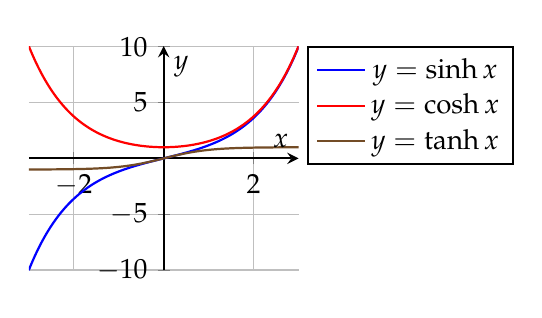
\begin{tikzpicture}
        \begin{axis}[
        scale = 0.5,
        xlabel={$x$},
        ylabel={$y$},
        axis lines=middle,
        samples=400,
        grid, thick, smooth,
        domain=- 3:3,
        legend pos=outer north east,
        ]
            \addplot+[no marks]{sinh(x)};
            \addlegendentry{$y = \sinh{x}$}
            \addplot+[no marks]{cosh(x)};
            \addlegendentry{$y = \cosh{x}$}
            \addplot+[no marks]{tanh(x)};
            \addlegendentry{$y = \tanh{x}$}
        \end{axis}
    \end{tikzpicture}

    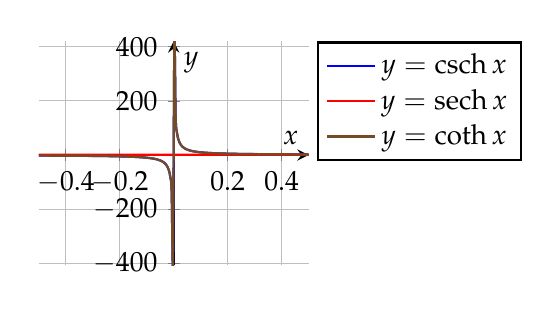
\begin{tikzpicture}
        \begin{axis}[
        scale = 0.5,
        xlabel={$x$},
        ylabel={$y$},
        axis lines=middle,
        samples=200,
        grid, thick, smooth,
        domain=- 0.5:0.5,
        legend pos=outer north east,
        ]
            \addplot+[no marks]{1 / sinh(x)};
            \addlegendentry{$y = \csch{x}$}
            \addplot+[no marks]{1 / cosh(x)};
            \addlegendentry{$y = \sech{x}$}
            \addplot+[no marks]{1 / tanh(x)};
            \addlegendentry{$y = \coth{x}$}
        \end{axis}
    \end{tikzpicture}

    \begin{displaymath}
        \arsinh{x} = \ln{(x + \sqrt{x^2 + 1})}
    \end{displaymath}

    \begin{displaymath}
        \arcosh{x} = \ln{(x \pm \sqrt{x^2 - 1})}
    \end{displaymath}

    \begin{displaymath}
        \artanh{x} = \frac{1}{2}\ln{(\frac{1 + x}{1 - x})}
    \end{displaymath}

    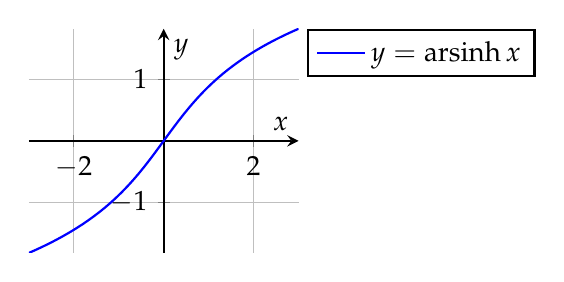
\begin{tikzpicture}
        \begin{axis}[
        scale = 0.5,
        xlabel={$x$},
        ylabel={$y$},
        axis lines=middle,
        samples=400,
        grid, thick, smooth,
        domain=- 3:3,
        legend pos=outer north east,
        ]
            \addplot+[no marks]{ln( x + sqrt(x^2 +1))};
            \addlegendentry{$y = \arsinh{x}$}
        \end{axis}
    \end{tikzpicture}

    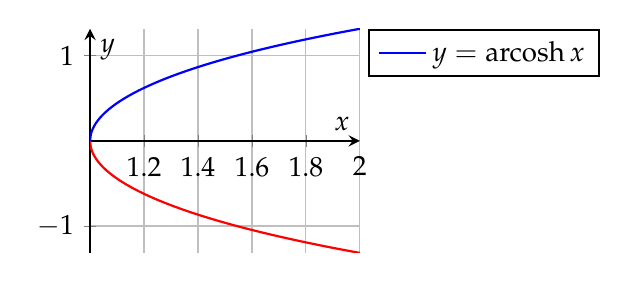
\begin{tikzpicture}
        \begin{axis}[
        scale = 0.5,
        xlabel={$x$},
        ylabel={$y$},
        axis lines=middle,
        samples=400,
        grid, thick, smooth,
        domain=1:2,
        legend pos=outer north east,
        ]
            \addplot+[no marks]{ln( x + sqrt(x^2 -1))};
            \addplot+[no marks]{ln( x - sqrt(x^2 -1))};
            \addlegendentry{$y = \arcosh{x}$}
        \end{axis}
    \end{tikzpicture}

    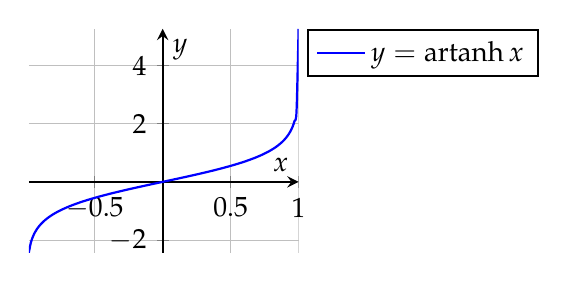
\begin{tikzpicture}
        \begin{axis}[
        scale = 0.5,
        xlabel={$x$},
        ylabel={$y$},
        axis lines=middle,
        samples=400,
        grid, thick, smooth,
        domain=- 3:3,
        legend pos=outer north east,
        ]
            \addplot+[no marks]{0.5*ln( (1+x)/(1-x))};
            \addlegendentry{$y = \artanh{x}$}
        \end{axis}
    \end{tikzpicture}

    \subsection{Osborn's rule}
    \textit{Replace $\sin$ with $\sinh$, $\cos$ with $\cosh$, $\sin^2$ with $-\sinh^2$}


    \section{Further coordinates}

    \subsection{Ellipses}

    \subsubsection{Standard equation}
    \begin{displaymath}
        \frac{x^2}{a^2} + \frac{y^2}{b^2} = 1
    \end{displaymath}

    \subsubsection{Parametric equation}

    \begin{displaymath}
        \left\{
        \begin{array}{c}
            x = a\cos\theta \\
            y = b\sin\theta
        \end{array}
    \end{displaymath}

    \subsubsection{Gradient of tangent for ellipse}

    \begin{displaymath}
        \frac{dy}{dx} = \frac{\frac{dy}{d\theta}}{\frac{dx}{d\theta}} = \frac{b\cos\theta}{-a\sin\theta} \\
    \end{displaymath}

    \subsection{Hyperbola}

    \begin{displaymath}
        \frac{x^2}{a^2} - \frac{y^2}{b^2} = 1
    \end{displaymath}

    \subsubsection{Asymptotes}
    \begin{displaymath}
        y = \pm\frac{b}{a}x
    \end{displaymath}

    \subsubsection{Intersections}
    \begin{displaymath}
        x = {\pm}a
    \end{displaymath}

    \subsubsection{Parametric equations}
    \begin{displaymath}
        \left\{
        \begin{array}{c}
            x = a\sec\theta \\
            y = b\tan\theta
        \end{array}
    \end{displaymath}
    \begin{displaymath}
        \left\{
        \begin{array}{c}
            x = a\cosh\theta \\
            y = b\sinh\theta
        \end{array}
    \end{displaymath}

    \subsubsection{Differentiation}
    \begin{displaymath}
        \frac{dy}{dx} = \frac{b}{a}\csc\theta
    \end{displaymath}

    \begin{displaymath}
        \frac{dy}{dx} = \frac{b}{a}\coth\theta
    \end{displaymath}

    \subsection{Eccentricity}

    \begin{displaymath}
        e = \frac{distance\ to\ focus}{distance\ to\ directrix}
    \end{displaymath}

    \begin{itemize}
        \item If $0 < e < 1$, it's an ellipse.
        $foci({\pm}ae, 0)$.
        directrix: $x = \pm\frac{a}{e}$
        \item If $e = 1$, it's an parabola.
    \end{itemize}

    \begin{figure}[!htb]
        \centering
        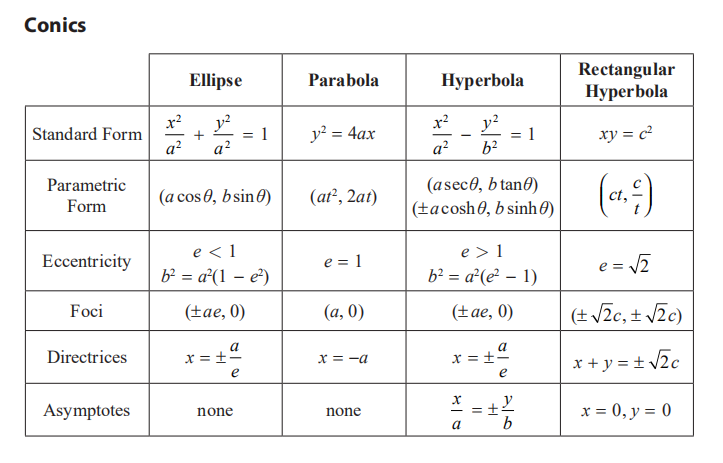
\includegraphics[width=0.7\textwidth]{Conics.png}
        % \caption{Full Rectification}
    \end{figure}

    Eccentricity for ellipse:

    \begin{displaymath}
        b^2 = a^2(1-e^2)
    \end{displaymath}

    \begin{displaymath}
        e^2 = 1 - \frac{b^2}{a^2}
    \end{displaymath}

    Eccentricity for hyperbola:

    \begin{displaymath}
        a^2 = b^2(1-e^2)
    \end{displaymath}

    \begin{displaymath}
        e^2 = 1 + \frac{b^2}{a^2}
    \end{displaymath}


    \section{Appendix: Formulas of Integration and Differentiation}

    \begin{displaymath}
        \int \frac{f'(x)}{f(x)} dx = \ln(f(x))
    \end{displaymath}

    \begin{displaymath}
        \sin^2(x) = \frac{1-\cos(2x)}{2}
    \end{displaymath}

    \begin{displaymath}
        \cos^2(x) = \frac{1+\cos(2x)}{2}
    \end{displaymath}

    \begin{displaymath}
        \int{\sec{x}}dx = \ln{(\sec{x} + \tan{x})} + C
    \end{displaymath}

    \begin{displaymath}
        \int{\csc{x}}dx = -\ln({\csc{x} + \cot{x}}) + C
    \end{displaymath}

    \begin{displaymath}
        \frac{d}{dx}(\sec{x}) = \sec{x}\tan{x}
    \end{displaymath}

    \begin{displaymath}
        \frac{d}{dx}(\tan{x}) = \sec^2{x}
    \end{displaymath}

    \begin{displaymath}
        \frac{d}{dx}(\cot{x}) = -\csc^2{x}
    \end{displaymath}

    \begin{displaymath}
        \frac{d}{dx}(\csc{x}) = -\csc{x}\cot{x}
    \end{displaymath}

\end{document}